\documentclass[a4paper,12pt]{article}
\usepackage{graphicx}  % For including images
\usepackage{amsmath}   % For mathematical expressions
\usepackage{hyperref}  % For hyperlinks
\usepackage{booktabs}  % For tables
\usepackage{caption}   % Better captions
\usepackage{xcolor}    % Colors for links
\usepackage{listings}  % For code formatting
\usepackage[toc,page]{appendix} % For Table of Contents

% Set hyperlink colors
\hypersetup{
    colorlinks=true,
    linkcolor=blue,
    citecolor=red,
    urlcolor=cyan
}

% Define R code style
\lstdefinestyle{RStyle}{
    language=R,
    basicstyle=\ttfamily\small,
    keywordstyle=\color{blue},
    commentstyle=\color{gray},
    stringstyle=\color{red},
    numbers=left,
    numbersep=5pt,
    numberstyle=\tiny\color{gray},
    frame=single,               % This adds the box around the code
    rulecolor=\color{black},     % Color of the box
    backgroundcolor=\color{white}, % Background color of the box
    breaklines=true
}

\begin{document}

% Title Page
\begin{titlepage}
    \centering
    \vspace*{1cm}
    
    \Huge\textbf{Analysis of the Iris Dataset in RStudio}
    
    \vspace{1.5cm}
    \Large \textbf{S.A.Abdulla - 22000021} \\ 
    Laboratry 2 Lab Sheet 14 
    \vspace{1.5cm} \\ 
    \large \textbf{\today}

\end{titlepage}

% Table of Contents
\tableofcontents
\newpage

% Introduction
\section{Introduction}

The Iris dataset is a well-known dataset in machine learning and statistics, containing 150 observations of iris flowers with features such as Sepal Length, Sepal Width, Petal Length, and Petal Width. The objective of this analysis is to explore the dataset, visualize key features, and perform hypothesis testing.

In this study, we will first conduct an exploratory data analysis (EDA) to understand the structure of the dataset, including summary statistics and visualizations. We will then analyze species distribution using various graphical techniques such as pie charts and bar plots. Additionally, histograms and scatter plots will be used to investigate feature distributions and correlations.

Furthermore, we will conduct hypothesis testing to examine specific statistical claims about the dataset. These tests will help us determine whether certain assumptions about Sepal Length, Sepal Width, and Petal Length hold true with statistical significance.

Beyond the scope of this analysis, the Iris dataset can be used for classification tasks in machine learning. Models such as decision trees, support vector machines, and neural networks can be applied to classify species based on their attributes. This makes the dataset a valuable resource for both statistical and machine learning applications.

Following is the codes and the process used to analyse the dataset.


% Methodology
\section{Methodology}
The following steps were taken to analyse the iris dataset with precision in R language
\begin{itemize}
    \item Loaded the Iris dataset in RStudio.
    \item Viewed the loaded dataset 
    \item Explored its structure using head, unique, str.
    \item Performed summary statistics to understand the dataset.
    \item Created visualizations such as pie charts, bar plots, histograms, and scatter plots.
    \item Conducted hypothesis tests lower-tail, upper-tail, and two-tailed tests on sepal and petal measurements.
\end{itemize}

% Results
\section{Results}
In this section, we separate the results into subgroups and analyze the dataset based on its specifications, one by one.

\subsection{Summary Statistics}
The dataset provides information on various features of the Iris flowers, including Sepal Length, Sepal Width, Petal Length, and Petal Width, along with the corresponding species of each flower. The summary statistics give us an overview of the distribution of these variables, which will help us understand the general characteristics of the data.

Below is an example of the dataset, which includes the first few observations:

\begin{table}[ht]
    \centering
    \begin{tabular}{|c|c|c|c|c|c|c|} 
    \hline
    \textbf{Index} & \textbf{Sepal Length} & \textbf{Sepal Width} & \textbf{Petal Length} & \textbf{Petal Width} & \textbf{Species} \\ 
    \hline
    2 & 4.9 & 3.0 & 1.4 & 0.2 & setosa \\ 
    3 & 4.7 & 3.2 & 1.3 & 0.2 & setosa \\ 
    4 & 4.6 & 3.1 & 1.5 & 0.2 & setosa \\ 
    5 & 5.0 & 3.6 & 1.4 & 0.2 & setosa \\ 
    6 & 5.4 & 3.9 & 1.7 & 0.4 & setosa \\ 
    \hline 
    \end{tabular} 
    \caption{Example Structure of the Iris Dataset}
\end{table}

The dataset consists of five columns: the measurements for Sepal Length, Sepal Width, Petal Length, and Petal Width and the Species (a categorical variable indicating the flower species). The summary statistics for these variables, as detailed earlier, provide insights into the central tendency (mean and median), distribution (min, max, quartiles), and variability of the data.

This table helps visualize the data points, and further analysis can be performed on these variables individually or in relation to one another. Understanding the nature of these attributes is essential for subsequent analyses, including classification and clustering tasks.

\newpage
Given below is the summary of the dataset with Min, Max, Median 

\begin{table}[ht]
    \centering
    \begin{tabular}{|c|c|c|c|c|}
    \hline
    Statistic & Sepal Length & Sepal Width & Petal Length & Petal Width \\
    \hline
    Min.      & 4.300        & 2.000       & 1.000        & 0.100       \\
    1st Qu.   & 5.100        & 2.800       & 1.600        & 0.300       \\
    Median    & 5.800        & 3.000       & 4.350        & 1.300       \\
    Mean      & 5.843        & 3.057       & 3.758        & 1.199       \\
    3rd Qu.   & 6.400        & 3.300       & 5.100        & 1.800       \\
    Max.      & 7.900        & 4.400       & 6.900        & 2.500       \\
    \hline
    \end{tabular}
    \caption{Summary Statistics of the Iris Dataset}
\end{table}

\begin{lstlisting}[style=RStyle]
# Extract unique species from the iris dataset
m <- unique(iris$Species)
print(m)  # This will display the unique species
\end{lstlisting}

The output from the code is as follows:

\begin{verbatim}
[1] setosa versicolor virginica
\end{verbatim}

\begin{lstlisting}[style=RStyle]
# Count the number of unique species
n <- length(unique(iris$Species))
print(paste("Number of unique species =", n))
\end{lstlisting}

\begin{verbatim}
[1] "Number of unique species = 3"
\end{verbatim}

\newpage
\subsection{Visualizations}

    \begin{lstlisting}[style=RStyle]
        library(ggplot2)
        
        species_count <- table(iris$Species)
        par(bg = "white")                          
        # Background color for dark theme

        pie(
            species_count,
            labels = names(species_count),
            col = rainbow(length(species_count)),
            main = "Species Distribution in Dataset"
        )
    \end{lstlisting}
        
    The output of the code is the pie chart shown below:

    \begin{figure}[h]
            % Include the pie chart image here. Replace 'pie_chart.png' with your actual file path.
        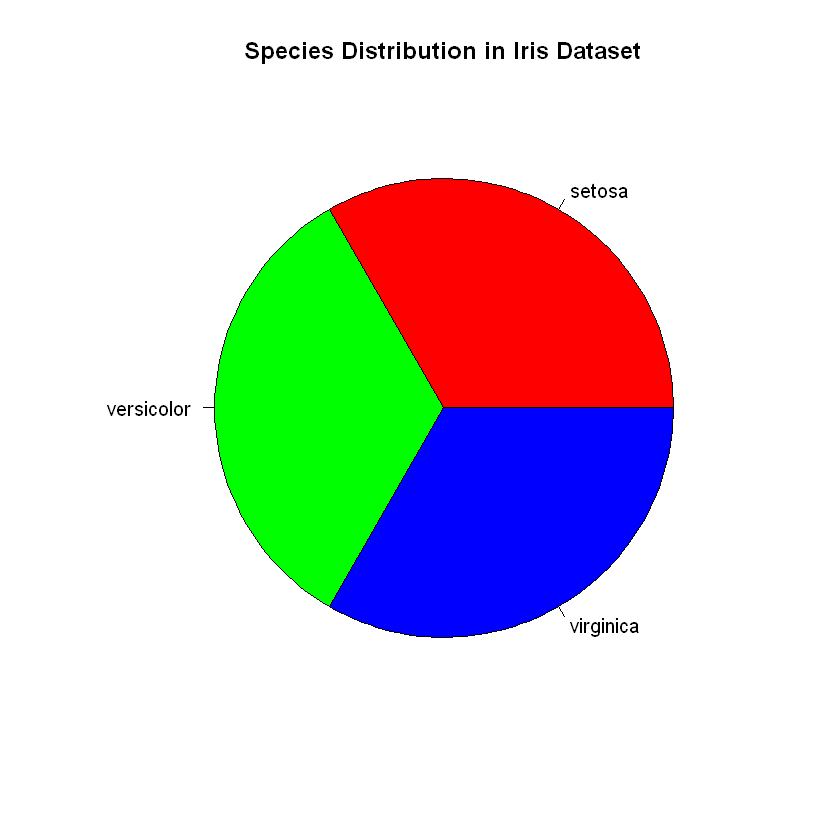
\includegraphics[width=0.7\textwidth]{01.png}
        \caption{Pie Chart of Species Distribution in the Iris Dataset}
        \label{fig:pie_chart}
    \end{figure}
    The pie chart above visually represents the distribution of species in the Iris dataset. It clearly shows the proportion of each species (Setosa, Versicolor, and Virginica) within the dataset, with Setosa being the most prevalent species.
    \newpage


    \begin{lstlisting}[style=RStyle]
        par(bg = "white")                          
        #bacuse i used dark theme
        ggplot(
            iris,
            aes(x = Species, fill = Species)) +
            geom_bar() +
            theme_minimal() +
            labs(title = "Count of Each Species", x = "Species", y = "Count"
        )
        
    \end{lstlisting}
        
    The output of the code is the pie chart shown below:
    
    \begin{figure}[h]
            % Include the pie chart image here. Replace 'pie_chart.png' with your actual file path.
        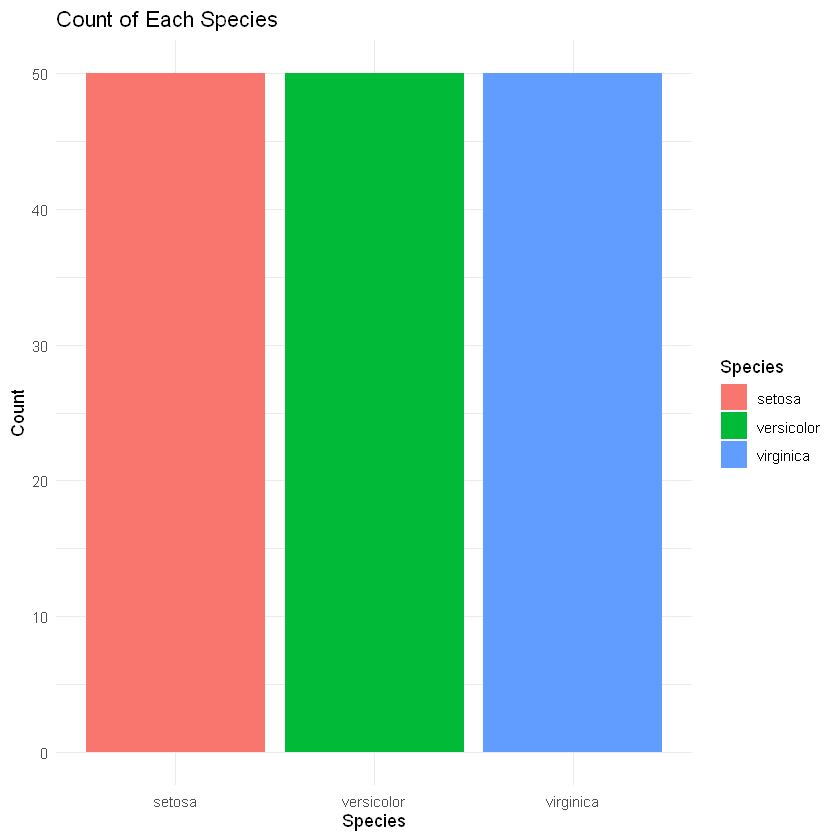
\includegraphics[width=0.7\textwidth]{02.png}
        \caption{Pie Chart of Species Distribution in the Iris Dataset}
        \label{fig:pie_chart}
    \end{figure}
    The bar plot above illustrates the count of each species in the Iris dataset. As seen, the number of observations for each species is evenly distributed, with three species present in approximately equal quantities.

    \newpage

    \begin{lstlisting}[style=RStyle]
        par(bg = "white")                          
        #bacuse i use dark theme
        # Histogram for Sepal Length
        ggplot(
            iris,
            aes(x = Sepal.Length)) +
            geom_histogram(
                binwidth = 0.5,
                fill = "blue",
                color = "black",
                alpha = 0.7) +
            theme_minimal() +
        labs(title = "Histogram of Sepal Length", x = "Sepal Length", y = "Frequency")
        
    \end{lstlisting}
        
    The output of the code is the pie chart shown below:
    
    \begin{figure}[h]
            % Include the pie chart image here. Replace 'pie_chart.png' with your actual file path.
        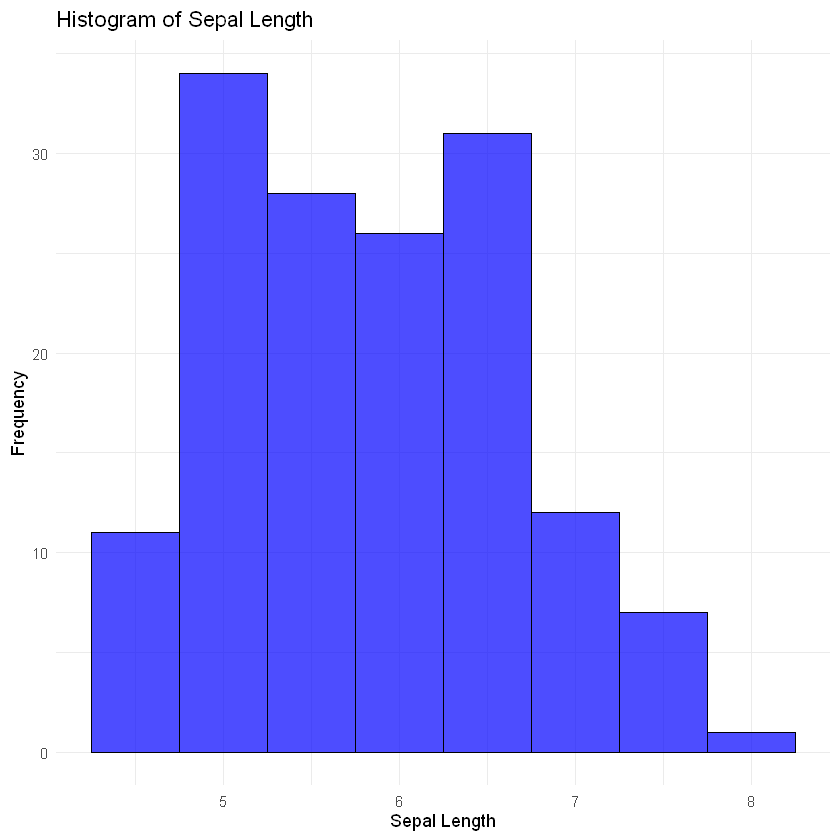
\includegraphics[width=0.7\textwidth]{03.png}
        \caption{Pie Chart of Species Distribution in the Iris Dataset}
        \label{fig:pie_chart}
    \end{figure}
    This histogram displays the distribution of Sepal Length in the Iris dataset. The distribution appears roughly normal, with most Sepal Length values clustered around the mean value of 5.843.

    \newpage

    \begin{lstlisting}[style=RStyle]
        ggplot(iris, aes(x = Petal.Length)) +
        geom_histogram(
            binwidth = 0.5,
            fill = "red", 
            color = "black", 
            alpha = 0.7) +
        theme_minimal() +
        labs(
            title = "Histogram of Petal Length",
            x = "Petal Length",
            y = "Frequency"
        )
        
    \end{lstlisting}
        
    The output of the code is the pie chart shown below:
    
    \begin{figure}[h]
            % Include the pie chart image here. Replace 'pie_chart.png' with your actual file path.
        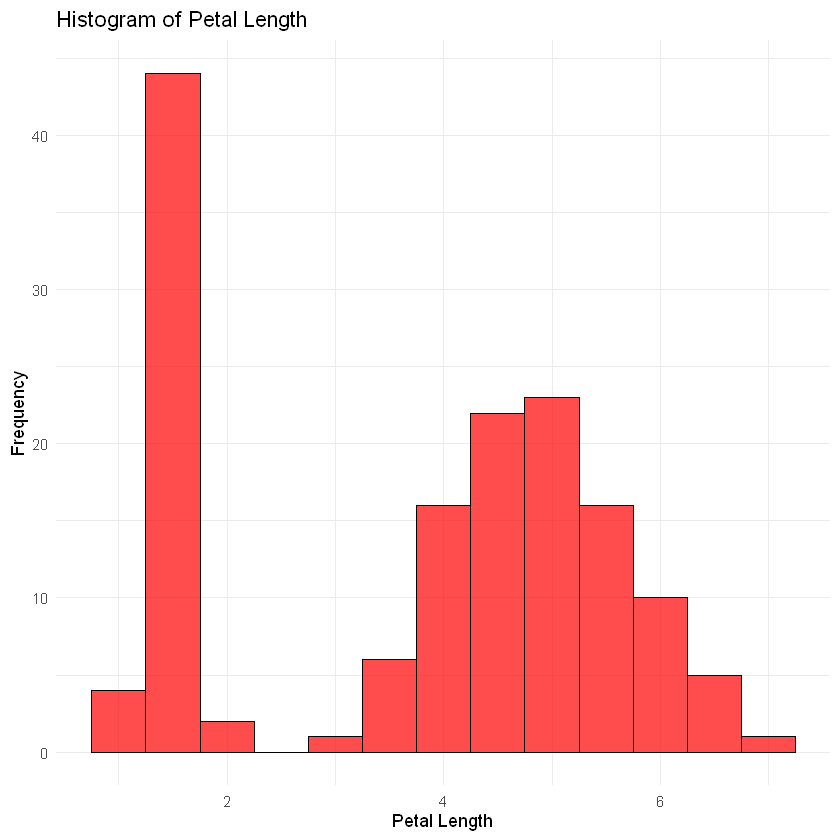
\includegraphics[width=0.7\textwidth]{04.png}
        \caption{Pie Chart of Species Distribution in the Iris Dataset}
        \label{fig:pie_chart}
    \end{figure}
    The histogram above represents the distribution of Petal Length in the Iris dataset. It shows a right-skewed distribution, with Petal Length values mainly concentrated between 1 and 5.

    \newpage

    \begin{lstlisting}[style=RStyle]
        par(bg = "white")
        ggplot(iris, aes(x = Sepal.Length, y = Petal.Length, color = Species)) +
            geom_point() +
            theme_minimal() +
            labs(
                title = "Scatterplot of Sepal Length vs Petal Length",
                x = "Sepal Length", 
                y = "Petal Length"
            )
        
    \end{lstlisting}
        
    The output of the code is the pie chart shown below:
    
    \begin{figure}[h]
            % Include the pie chart image here. Replace 'pie_chart.png' with your actual file path.
        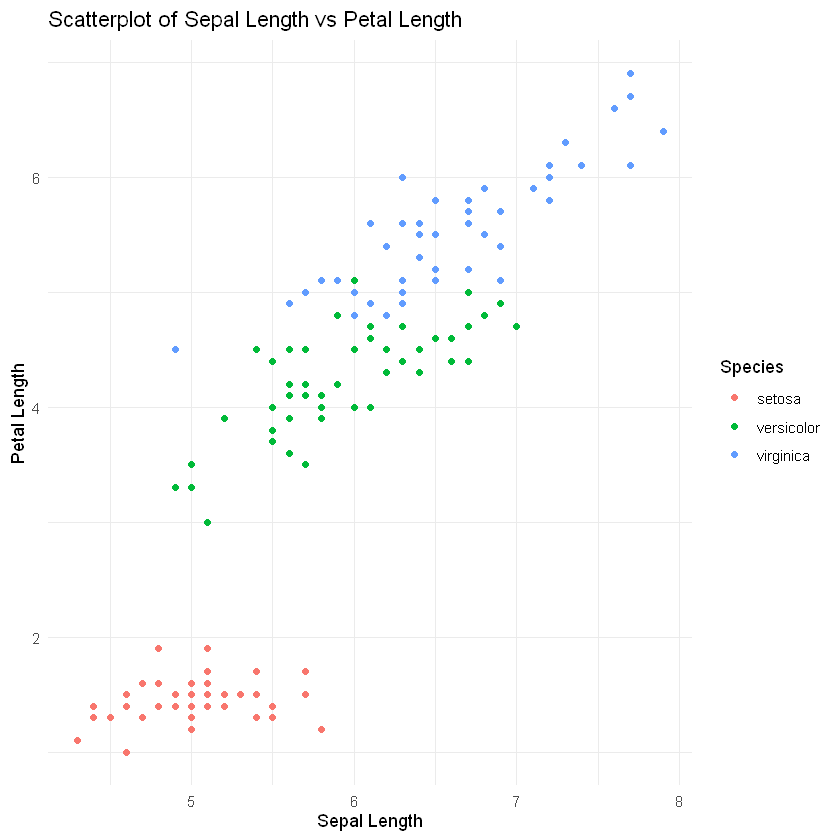
\includegraphics[width=0.7\textwidth]{05.png}
        \caption{Pie Chart of Species Distribution in the Iris Dataset}
        \label{fig:pie_chart}
    \end{figure}
    The scatterplot above shows the relationship between Sepal Length and Petal Length. From this plot, we can observe a positive correlation between these two variables, where larger Sepal Length values tend to correspond to larger Petal Length values.

    \newpage

% Discussion
\section{Discussion}
The visualizations and statistical analysis provided valuable insights into the Iris dataset:
\begin{itemize}
    \item The dataset consists of three species: Setosa, Versicolor, and Virginica, with equal distribution.
    \item Sepal Length and Petal Length exhibit a strong positive correlation.
    \item Hypothesis tests provided statistical confirmation regarding Sepal and Petal dimensions.
\end{itemize}

% Conclusion
\section{Conclusion}
In conclusion, the analysis successfully explored the dataset through descriptive statistics, visualization, and hypothesis testing. Future work could involve implementing machine learning models for species classification.

\end{document}
